\documentclass[a4paper, 12pt]{article}
\usepackage{standardopsætning}

%----------------------------------------------------------------
%   HEADER & FOOTER
%----------------------------------------------------------------

\pagestyle{fancy}
\fancyhf{} % Nulstil alle header og footer felter
\lhead{Dit Navn}
\chead{Fag: Mit Fag}
\rhead{Dato: \today}
\rfoot{Side \thepage\ af \pageref*{LastPage}}

%----------------------------------------------------------------
%   TITEL INFORMATION
%----------------------------------------------------------------

\title{Titel på Aflevering}
\author{Dit Navn \\ Mit Fag}
\date{\today}

%----------------------------------------------------------------
%   DOKUMENT START
%----------------------------------------------------------------

\begin{document}

\maketitle
\thispagestyle{empty} % No header/footer on the title page
\newpage
\setcounter{page}{1}

%----------------------------------------------------------------
%   INDHOLDSFORTEGNELSE (OPTIONEL)
%----------------------------------------------------------------

%\tableofcontents
%%\listoffigures
%%\listoftables
%\newpage

%----------------------------------------------------------------
%   DOKUMENTINDHOLD
%----------------------------------------------------------------

\section{Opgave 1}
\subsection*{Spørgsmål 1.1}
Her er løsningen til den første opgave. Man kan bruge \texttt{amsmath} til at skrive komplekse ligninger som denne:
$$
E = mc^2
$$
Eller et integral:
$$
\int_{a}^{b} x^2 \,dx
$$
\begin{figure}[h!]
    \centering
    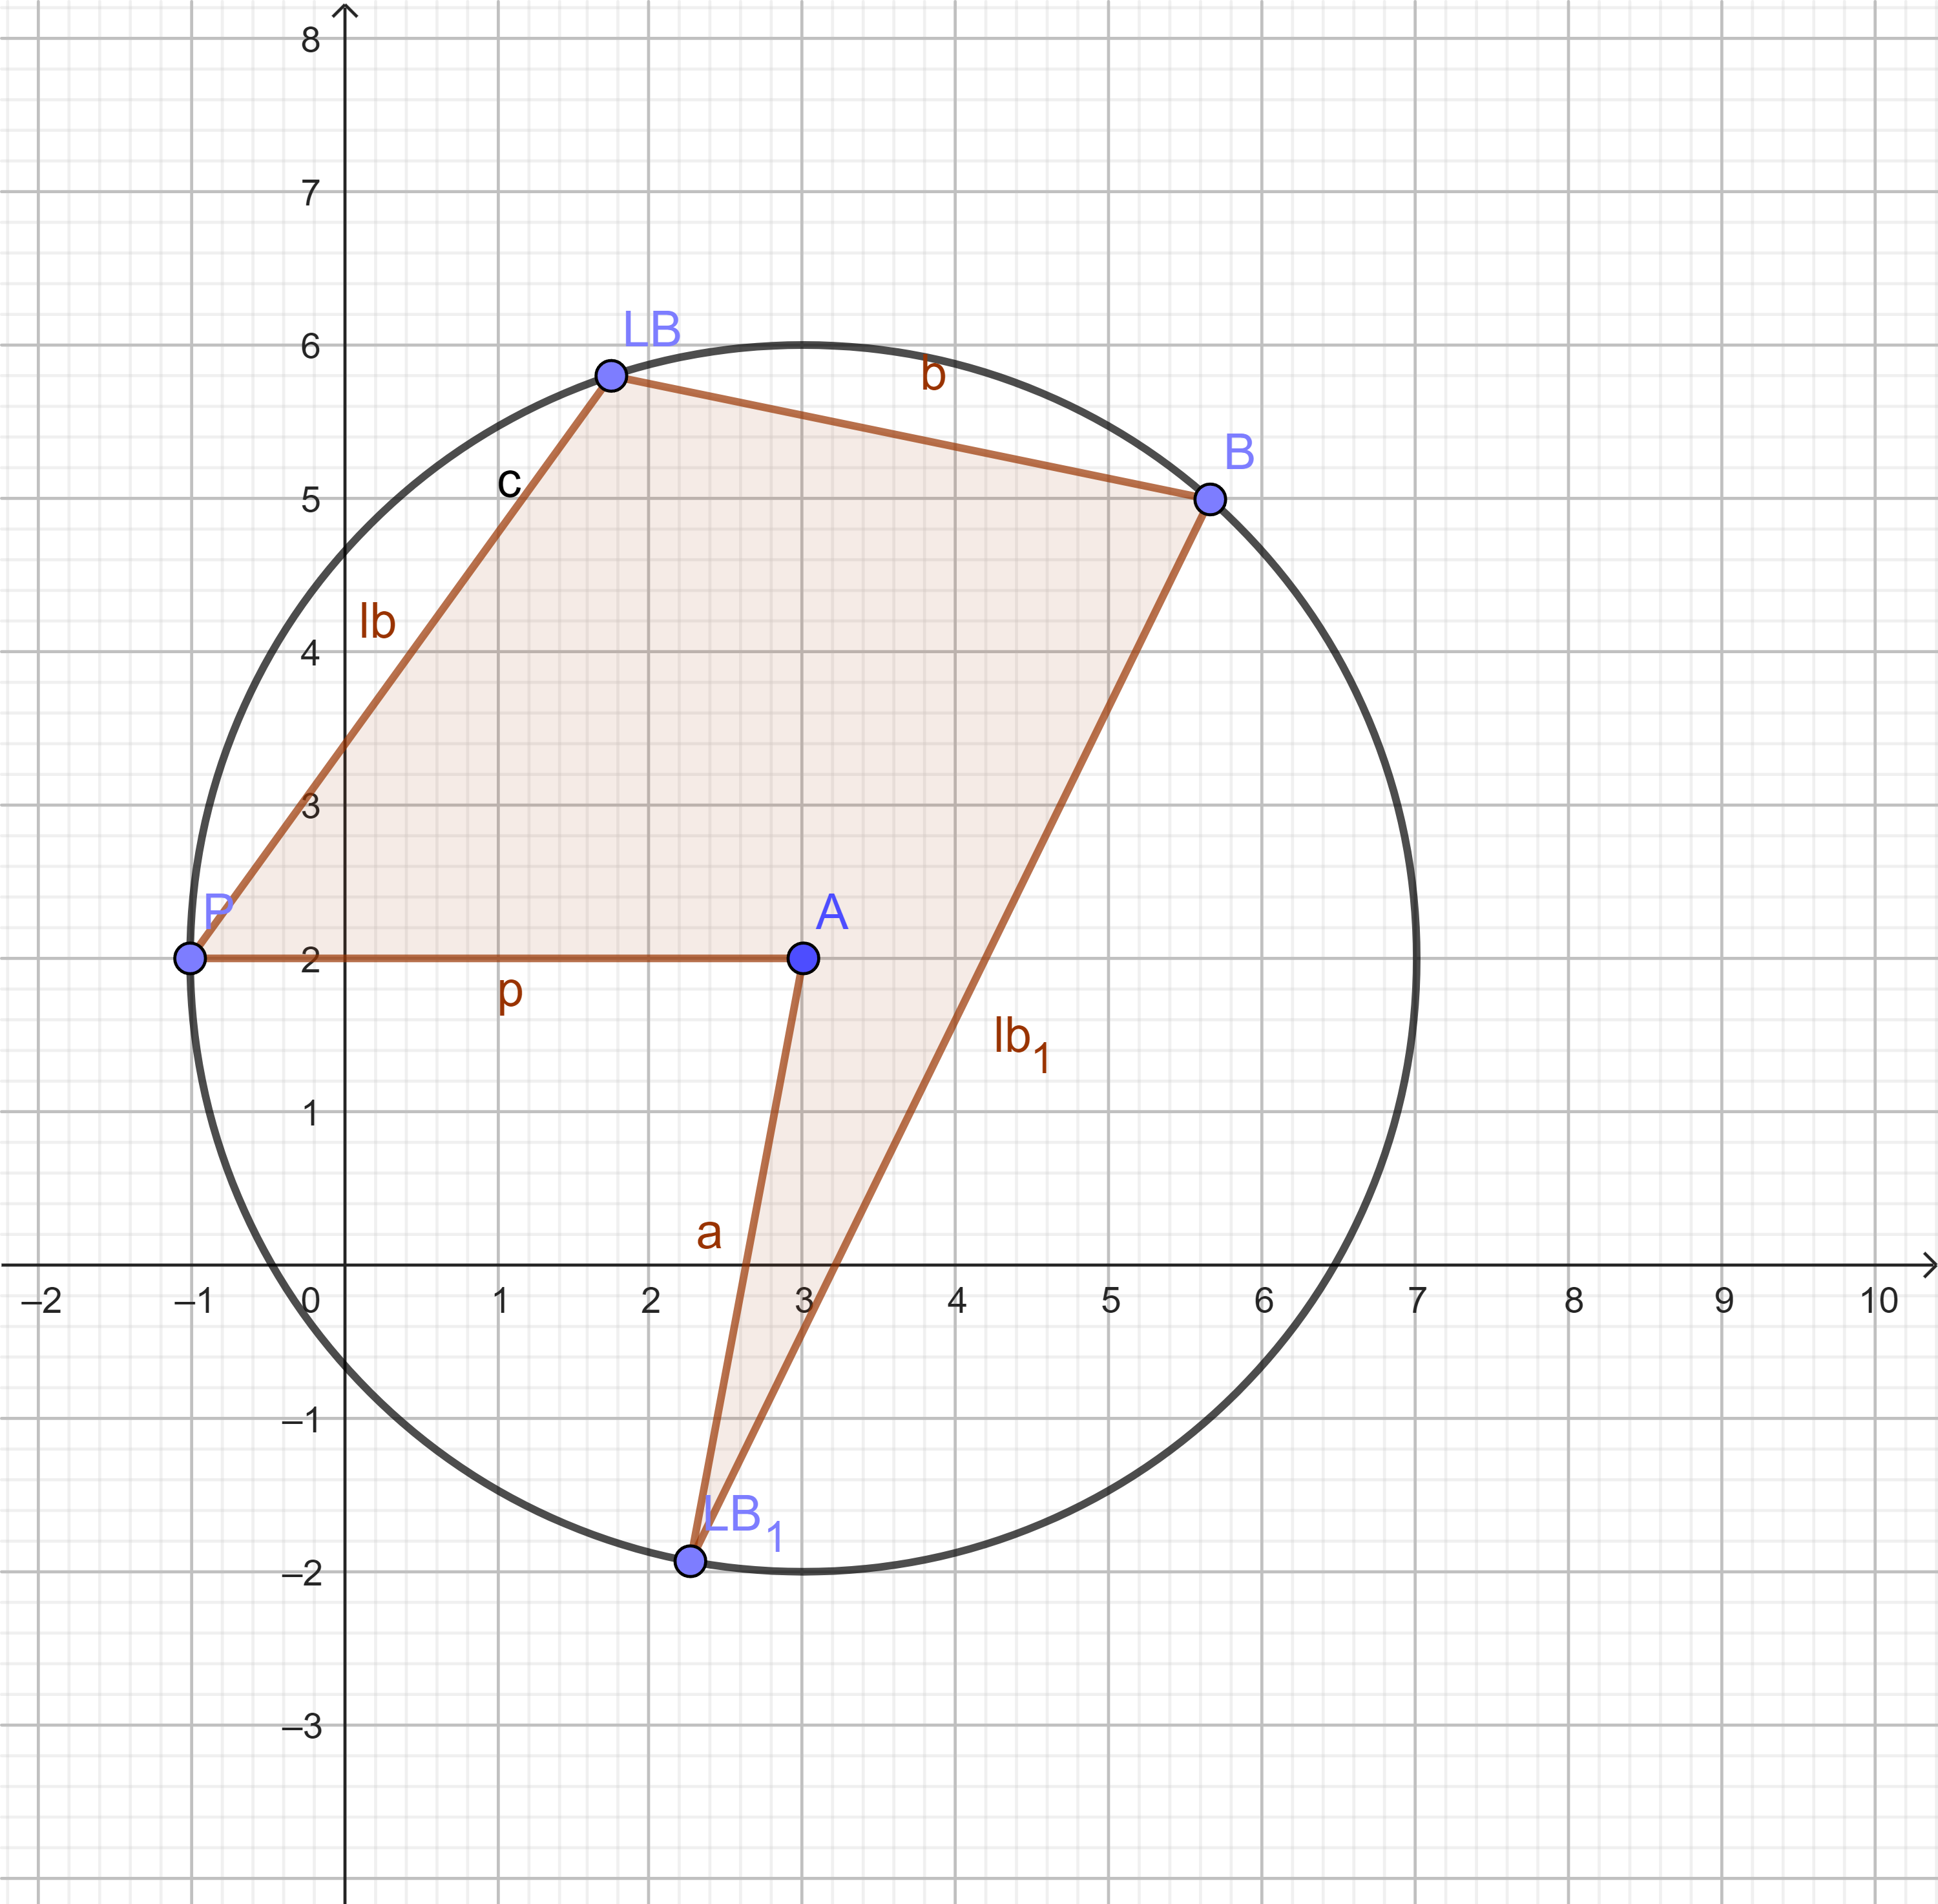
\includegraphics[width = 0.65\textwidth]{geogebra-polyg.png}
    \caption[List of Figures tekst (\texttt{\ listoffigures})]{Irregulær polygon. Oprettet med \url{https://www.geogebra.org/}} \href{https://www.geogebra.org/}{Geogebra} kan gratis anvendes til både undervisning, tekniske tegninger og geometriske udregninger i 2D og 3D.
    \label{fig:geog-poly1}
\end{figure}

Man kan også bruge \texttt{siunitx} til at formatere enheder korrekt. For eksempel er tyngdeaccelerationen på Jorden cirka \SI{9.82}{\meter\newton\cubed\per\second\squared\kg}.

\section{Opgave 2}

I denne opgave indsættes et billede og en tabel.

\begin{figure}[h!t]
  \centering
  % \includegraphics[width=0.8\textwidth]{billedenavn} % Uncomment to insert an image
  \caption{Dette er en figur. Takket være \texttt{babel} og \texttt{cleveref}, kan vi referere til den som \cref{fig:geog-poly1}.}
  \label{fig:eksempel}
\end{figure}

\begin{sætning}
\label{kont}
Let \(f\) be a function whose derivative exists in every point, then \(f\) is 
a continuous function.
\end{sætning}
Her er en tabel lavet med \texttt{booktabs}:

\begin{table}[h!]
  \caption{En tabel med eksempler på massefylder. Vi kan referere til den som \cref{tab:massefylder}.}
  \label{tab:massefylder}
  \centering
  \begin{tabular}{l c r}
    \toprule
    \textbf{Materiale} & \textbf{Symbol} & \textbf{Massefylde (\si{\kilo\gram\per\cubic\meter})} \\
    \midrule
    Vand & \ce{H2O} & \num{1000} \\
    Jern & \ce{Fe} & \num{7874} \\
    Guld & \ce{Au} & \num{19300} \\
    Henfald & \ce{^234_90Th -> ^0_-1\beta{} + ^234_91Pa} & \qty{1164562.554978}{\litre.\km\per\newton\squared.\second^{3.5}} \\
    \bottomrule
  \end{tabular}
\end{table}

\begin{sætning}[Pythagorean theorem]
\label{pythagorean}
This is a theorem about right triangles and can be summarised in the next 
equation 
\[ x^2 + y^2 = z^2 \]
\end{sætning}
\begin{sætning}[Pythagorean theorem]
\label{pythagoreandk}
Denne sætning er på dansk:
\[ x^2 + y^2 = z^2 \]
som også nogen gange ses som
\begin{equation}\label{abc}
    a^2 + b^2 = c^2
\end{equation}
\end{sætning}
Som det ses i \cref{tab:massefylder}, er guld meget tungere end vand.

\begin{korollar}
There's no right rectangle whose sides measure 3cm, 4cm, and 6cm.
\end{korollar}

Dette ses fra \cref{kont} og, del dels også fra \Cref{pythagorean}.

Nu kigger vi på \Cref{kont,pythagorean,pythagoreandk}, \cref{abc} og \cref{tab:massefylder} versus \Cref{kont} og \Cref{pythagorean}\footnote{\cite{greenwade93}}.

\begin{lemma}
Given two line segments whose lengths are \(a\) and \(b\) respectively there is a 
real number \(r\) such that \(b=ra\).
\end{lemma}

\section*{Konklusion}
Dette er en konklusion på opgavesættet. Se lige den flotte figur igen: \cref{fig:geog-poly1}!

Men vi er også nødt til at tale om et sæt af ligninger:
\begin{alignat*}{2}
    f(x) &= \left(x+\frac{y}{z}\right)+89 &\Leftrightarrow \\
    g(x) &= x=6                           &\Leftrightarrow \\
    h(x) &= \qty{8912342.6712332}{\km.\second\per\newton\squared\pascal}
\end{alignat*}
versus
\begin{alignat}{3}
    & f(x) && = \left(x+\frac{y}{z}\right)+89 && \Leftrightarrow\label{eq:fst} \\
    & g(x) && = \frac{\displaystyle\int^\frac{x^2-2x}{a^2-\sqrt{4ac}}_{\sqrt[6]{\frac{y^2+z^2}{x^2}}}x^4+y^6+z^8\dd x\dd y\dd z}{2x-4y+3z=0}=6  && \Leftrightarrow\label{eq:mid} \\
    & h(x) && = \qty{8912342.6712332}{\km.\second\per\newton\squared\pascal}\notag
\end{alignat}
Vi vi gerne vil fremhæve \cref{eq:fst,eq:mid} som de vigtigste.
\label{LastPage} % Used for the "Side X af Y" footer
\newpage
\bibliographystyle{alpha}
\bibliography{sample}
\end{document}